\documentclass[journal]{IEEEtran}
\usepackage{blindtext}
\usepackage{graphicx}
\documentclass{amsart}
\documentclass{article}
\usepackage{amsmath}
% *** CITATION PACKAGES ***
%
%\usepackage{cite}
% cite.sty was written by Donald Arseneau
% V1.6 and later of IEEEtran pre-defines the format of the cite.sty package
% \cite{} output to follow that of IEEE. Loading the cite package will
% result in citation numbers being automatically sorted and properly
% "compressed/ranged". e.g., [1], [9], [2], [7], [5], [6] without using
% cite.sty will become [1], [2], [5]--[7], [9] using cite.sty. cite.sty's
% \cite will automatically add leading space, if needed. Use cite.sty's
% noadjust option (cite.sty V3.8 and later) if you want to turn this off.
% cite.sty is already installed on most LaTeX systems. Be sure and use
% version 4.0 (2003-05-27) and later if using hyperref.sty. cite.sty does
% not currently provide for hyperlinked citations.
% The latest version can be obtained at:
% http://www.ctan.org/tex-archive/macros/latex/contrib/cite/
% The documentation is contained in the cite.sty file itself.

% *** GRAPHICS RELATED PACKAGES ***
%
\ifCLASSINFOpdf
  % \usepackage[pdftex]{graphicx}
  % declare the path(s) where your graphic files are
  % \graphicspath{{../pdf/}{../jpeg/}}
  % and their extensions so you won't have to specify these with
  % every instance of \includegraphics
  % \DeclareGraphicsExtensions{.pdf,.jpeg,.png}
\else
  % or other class option (dvipsone, dvipdf, if not using dvips). graphicx
  % will default to the driver specified in the system graphics.cfg if no
  % driver is specified.
  % \usepackage[dvips]{graphicx}
  % declare the path(s) where your graphic files are
  % \graphicspath{{../eps/}}
  % and their extensions so you won't have to specify these with
  % every instance of \includegraphics
  % \DeclareGraphicsExtensions{.eps}
\fi
% graphicx was written by David Carlisle and Sebastian Rahtz. It is
% required if you want graphics, photos, etc. graphicx.sty is already
% installed on most LaTeX systems. The latest version and documentation can
% be obtained at: 
% http://www.ctan.org/tex-archive/macros/latex/required/graphics/
% Another good source of documentation is "Using Imported Graphics in
% LaTeX2e" by Keith Reckdahl which can be found as epslatex.ps or
% epslatex.pdf at: http://www.ctan.org/tex-archive/info/
%
% latex, and pdflatex in dvi mode, support graphics in encapsulated
% postscript (.eps) format. pdflatex in pdf mode supports graphics
% in .pdf, .jpeg, .png and .mps (metapost) formats. Users should ensure
% that all non-photo figures use a vector format (.eps, .pdf, .mps) and
% not a bitmapped formats (.jpeg, .png). IEEE frowns on bitmapped formats
% which can result in "jaggedy"/blurry rendering of lines and letters as
% well as large increases in file sizes.
%
% You can find documentation about the pdfTeX application at:
% http://www.tug.org/applications/pdftex





% *** MATH PACKAGES ***
%
%\usepackage[cmex10]{amsmath}
% A popular package from the American Mathematical Society that provides
% many useful and powerful commands for dealing with mathematics. If using
% it, be sure to load this package with the cmex10 option to ensure that
% only type 1 fonts will utilized at all point sizes. Without this option,
% it is possible that some math symbols, particularly those within
% footnotes, will be rendered in bitmap form which will result in a
% document that can not be IEEE Xplore compliant!
%
% Also, note that the amsmath package sets \interdisplaylinepenalty to 10000
% thus preventing page breaks from occurring within multiline equations. Use:
%\interdisplaylinepenalty=2500
% after loading amsmath to restore such page breaks as IEEEtran.cls normally
% does. amsmath.sty is already installed on most LaTeX systems. The latest
% version and documentation can be obtained at:
% http://www.ctan.org/tex-archive/macros/latex/required/amslatex/math/





% *** SPECIALIZED LIST PACKAGES ***
%
%\usepackage{algorithmic}
% algorithmic.sty was written by Peter Williams and Rogerio Brito.
% This package provides an algorithmic environment fo describing algorithms.
% You can use the algorithmic environment in-text or within a figure
% environment to provide for a floating algorithm. Do NOT use the algorithm
% floating environment provided by algorithm.sty (by the same authors) or
% algorithm2e.sty (by Christophe Fiorio) as IEEE does not use dedicated
% algorithm float types and packages that provide these will not provide
% correct IEEE style captions. The latest version and documentation of
% algorithmic.sty can be obtained at:
% http://www.ctan.org/tex-archive/macros/latex/contrib/algorithms/
% There is also a support site at:
% http://algorithms.berlios.de/index.html
% Also of interest may be the (relatively newer and more customizable)
% algorithmicx.sty package by Szasz Janos:
% http://www.ctan.org/tex-archive/macros/latex/contrib/algorithmicx/




% *** ALIGNMENT PACKAGES ***
%
%\usepackage{array}
% Frank Mittelbach's and David Carlisle's array.sty patches and improves
% the standard LaTeX2e array and tabular environments to provide better
% appearance and additional user controls. As the default LaTeX2e table
% generation code is lacking to the point of almost being broken with
% respect to the quality of the end results, all users are strongly
% advised to use an enhanced (at the very least that provided by array.sty)
% set of table tools. array.sty is already installed on most systems. The
% latest version and documentation can be obtained at:
% http://www.ctan.org/tex-archive/macros/latex/required/tools/


%\usepackage{mdwmath}
%\usepackage{mdwtab}
% Also highly recommended is Mark Wooding's extremely powerful MDW tools,
% especially mdwmath.sty and mdwtab.sty which are used to format equations
% and tables, respectively. The MDWtools set is already installed on most
% LaTeX systems. The lastest version and documentation is available at:
% http://www.ctan.org/tex-archive/macros/latex/contrib/mdwtools/


% IEEEtran contains the IEEEeqnarray family of commands that can be used to
% generate multiline equations as well as matrices, tables, etc., of high
% quality.


%\usepackage{eqparbox}
% Also of notable interest is Scott Pakin's eqparbox package for creating
% (automatically sized) equal width boxes - aka "natural width parboxes".
% Available at:
% http://www.ctan.org/tex-archive/macros/latex/contrib/eqparbox/





% *** SUBFIGURE PACKAGES ***
%\usepackage[tight,footnotesize]{subfigure}
% subfigure.sty was written by Steven Douglas Cochran. This package makes it
% easy to put subfigures in your figures. e.g., "Figure 1a and 1b". For IEEE
% work, it is a good idea to load it with the tight package option to reduce
% the amount of white space around the subfigures. subfigure.sty is already
% installed on most LaTeX systems. The latest version and documentation can
% be obtained at:
% http://www.ctan.org/tex-archive/obsolete/macros/latex/contrib/subfigure/
% subfigure.sty has been superceeded by subfig.sty.



%\usepackage[caption=false]{caption}
%\usepackage[font=footnotesize]{subfig}
% subfig.sty, also written by Steven Douglas Cochran, is the modern
% replacement for subfigure.sty. However, subfig.sty requires and
% automatically loads Axel Sommerfeldt's caption.sty which will override
% IEEEtran.cls handling of captions and this will result in nonIEEE style
% figure/table captions. To prevent this problem, be sure and preload
% caption.sty with its "caption=false" package option. This is will preserve
% IEEEtran.cls handing of captions. Version 1.3 (2005/06/28) and later 
% (recommended due to many improvements over 1.2) of subfig.sty supports
% the caption=false option directly:
%\usepackage[caption=false,font=footnotesize]{subfig}
%
% The latest version and documentation can be obtained at:
% http://www.ctan.org/tex-archive/macros/latex/contrib/subfig/
% The latest version and documentation of caption.sty can be obtained at:
% http://www.ctan.org/tex-archive/macros/latex/contrib/caption/




% *** FLOAT PACKAGES ***
%
%\usepackage{fixltx2e}
% fixltx2e, the successor to the earlier fix2col.sty, was written by
% Frank Mittelbach and David Carlisle. This package corrects a few problems
% in the LaTeX2e kernel, the most notable of which is that in current
% LaTeX2e releases, the ordering of single and double column floats is not
% guaranteed to be preserved. Thus, an unpatched LaTeX2e can allow a
% single column figure to be placed prior to an earlier double column
% figure. The latest version and documentation can be found at:
% http://www.ctan.org/tex-archive/macros/latex/base/



%\usepackage{stfloats}
% stfloats.sty was written by Sigitas Tolusis. This package gives LaTeX2e
% the ability to do double column floats at the bottom of the page as well
% as the top. (e.g., "\begin{figure*}[!b]" is not normally possible in
% LaTeX2e). It also provides a command:
%\fnbelowfloat
% to enable the placement of footnotes below bottom floats (the standard
% LaTeX2e kernel puts them above bottom floats). This is an invasive package
% which rewrites many portions of the LaTeX2e float routines. It may not work
% with other packages that modify the LaTeX2e float routines. The latest
% version and documentation can be obtained at:
% http://www.ctan.org/tex-archive/macros/latex/contrib/sttools/
% Documentation is contained in the stfloats.sty comments as well as in the
% presfull.pdf file. Do not use the stfloats baselinefloat ability as IEEE
% does not allow \baselineskip to stretch. Authors submitting work to the
% IEEE should note that IEEE rarely uses double column equations and
% that authors should try to avoid such use. Do not be tempted to use the
% cuted.sty or midfloat.sty packages (also by Sigitas Tolusis) as IEEE does
% not format its papers in such ways.


%\ifCLASSOPTIONcaptionsoff
%  \usepackage[nomarkers]{endfloat}
% \let\MYoriglatexcaption\caption
% \renewcommand{\caption}[2][\relax]{\MYoriglatexcaption[#2]{#2}}
%\fi
% endfloat.sty was written by James Darrell McCauley and Jeff Goldberg.
% This package may be useful when used in conjunction with IEEEtran.cls'
% captionsoff option. Some IEEE journals/societies require that submissions
% have lists of figures/tables at the end of the paper and that
% figures/tables without any captions are placed on a page by themselves at
% the end of the document. If needed, the draftcls IEEEtran class option or
% \CLASSINPUTbaselinestretch interface can be used to increase the line
% spacing as well. Be sure and use the nomarkers option of endfloat to
% prevent endfloat from "marking" where the figures would have been placed
% in the text. The two hack lines of code above are a slight modification of
% that suggested by in the endfloat docs (section 8.3.1) to ensure that
% the full captions always appear in the list of figures/tables - even if
% the user used the short optional argument of \caption[]{}.
% IEEE papers do not typically make use of \caption[]'s optional argument,
% so this should not be an issue. A similar trick can be used to disable
% captions of packages such as subfig.sty that lack options to turn off
% the subcaptions:
% For subfig.sty:
% \let\MYorigsubfloat\subfloat
% \renewcommand{\subfloat}[2][\relax]{\MYorigsubfloat[]{#2}}
% For subfigure.sty:
% \let\MYorigsubfigure\subfigure
% \renewcommand{\subfigure}[2][\relax]{\MYorigsubfigure[]{#2}}
% However, the above trick will not work if both optional arguments of
% the \subfloat/subfig command are used. Furthermore, there needs to be a
% description of each subfigure *somewhere* and endfloat does not add
% subfigure captions to its list of figures. Thus, the best approach is to
% avoid the use of subfigure captions (many IEEE journals avoid them anyway)
% and instead reference/explain all the subfigures within the main caption.
% The latest version of endfloat.sty and its documentation can obtained at:
% http://www.ctan.org/tex-archive/macros/latex/contrib/endfloat/
%
% The IEEEtran \ifCLASSOPTIONcaptionsoff conditional can also be used
% later in the document, say, to conditionally put the References on a 
% page by themselves.





% *** PDF, URL AND HYPERLINK PACKAGES ***
%
%\usepackage{url}
% url.sty was written by Donald Arseneau. It provides better support for
% handling and breaking URLs. url.sty is already installed on most LaTeX
% systems. The latest version can be obtained at:
% http://www.ctan.org/tex-archive/macros/latex/contrib/misc/
% Read the url.sty source comments for usage information. Basically,
% \url{my_url_here}.





% *** Do not adjust lengths that control margins, column widths, etc. ***
% *** Do not use packages that alter fonts (such as pslatex).         ***
% There should be no need to do such things with IEEEtran.cls V1.6 and later.
% (Unless specifically asked to do so by the journal or conference you plan
% to submit to, of course. )


% correct bad hyphenation here
\hyphenation{op-tical net-works semi-conduc-tor}


\begin{document}
%
% paper title
% can use linebreaks \\ within to get better formatting as desired
\title{Signals and Systems Project 2 Report}
%
%
% author names and IEEE memberships
% note positions of commas and nonbreaking spaces ( ~ ) LaTeX will not break
% a structure at a ~ so this keeps an author's name from being broken across
% two lines.
% use \thanks{} to gain access to the first footnote area
% a separate \thanks must be used for each paragraph as LaTeX2e's \thanks
% was not built to handle multiple paragraphs
%

\author{Cheng-I Lai}%
        % John~Doe,~\IEEEmembership{Fellow,~OSA,}
        % and~Jane~Doe,~\IEEEmembership{Life~Fellow,~IEEE}% <-this % stops a space
% \thanks{M. Shell is with the Department
% of Electrical and Computer Engineering, Georgia Institute of Technology, Atlanta,
% GA, 30332 USA e-mail: (see http://www.michaelshell.org/contact.html).}% <-this % stops a space
% \thanks{J. Doe and J. Doe are with Anonymous University.}% <-this % stops a space
% \thanks{Manuscript received April 19, 2005; revised January 11, 2007.}}

% note the % following the last \IEEEmembership and also \thanks - 
% these prevent an unwanted space from occurring between the last author name
% and the end of the author line. i.e., if you had this:
% 
% \author{....lastname \thanks{...} \thanks{...} }
%                     ^------------^------------^----Do not want these spaces!
%
% a space would be appended to the last name and could cause every name on that
% line to be shifted left slightly. This is one of those "LaTeX things". For
% instance, "\textbf{A} \textbf{B}" will typeset as "A B" not "AB". To get
% "AB" then you have to do: "\textbf{A}\textbf{B}"
% \thanks is no different in this regard, so shield the last } of each \thanks
% that ends a line with a % and do not let a space in before the next \thanks.
% Spaces after \IEEEmembership other than the last one are OK (and needed) as
% you are supposed to have spaces between the names. For what it is worth,
% this is a minor point as most people would not even notice if the said evil
% space somehow managed to creep in.



% The paper headers
\markboth{\today}%
{Shell \MakeLowercase{\textit{et al.}}: Bare Demo of IEEEtran.cls for Journals}
% The only time the second header will appear is for the odd numbered pages
% after the title page when using the twoside option.
% 
% *** Note that you probably will NOT want to include the author's ***
% *** name in the headers of peer review papers.                   ***
% You can use \ifCLASSOPTIONpeerreview for conditional compilation here if
% you desire.




% If you want to put a publisher's ID mark on the page you can do it like
% this:
%\IEEEpubid{0000--0000/00\$00.00~\copyright~2007 IEEE}
% Remember, if you use this you must call \IEEEpubidadjcol in the second
% column for its text to clear the IEEEpubid mark.



% use for special paper notices
%\IEEEspecialpapernotice{(Invited Paper)}




% make the title area
\maketitle


\begin{abstract}
%\boldmath
Speech Denoising, or noise cancellation, is a technique to produce a better quality signal given a noisy input signal. This technique is significant for its wide application in speech recognition or detection. Specifically, we tackle speech signals mixed with different kinds of noise, such as white noise. Applying Fourier transform with spectral subtraction attains our goal. In this paper, we will implement two kinds of noise cancellation systems, visualize their results, and analyze the effects of different kinds of noise. At the end, readers should obtain a general concept of simple noise cancellation techniques. 

\end{abstract}
% IEEEtran.cls defaults to using nonbold math in the Abstract.
% This preserves the distinction between vectors and scalars. However,
% if the journal you are submitting to favors bold math in the abstract,
% then you can use LaTeX's standard command \boldmath at the very start
% of the abstract to achieve this. Many IEEE journals frown on math
% in the abstract anyway.

% Note that keywords are not normally used for peerreview papers.
\begin{IEEEkeywords}
Signals and Systems, Speech Denoising, Spectrum Analysis, Fourier Analysis 
\end{IEEEkeywords}






% For peer review papers, you can put extra information on the cover
% page as needed:
% \ifCLASSOPTIONpeerreview
% \begin{center} \bfseries EDICS Category: 3-BBND \end{center}
% \fi
%
% For peerreview papers, this IEEEtran command inserts a page break and
% creates the second title. It will be ignored for other modes.
% \IEEEpeerreviewmaketitle

\section{Introduction}
\begin{flushleft}
The experiment setup can be summarize as the diagram below. The input signal x(t) is analyzed over short segments by dividing it into frames and classifying each frame as speech or noise. If the segment is noise, we compute its magnitude spectrum $|N_\omega(\omega)|$ and average $|N_\omega(\omega)|$ over all noise frames. If the segment is speech, we extract both of its magnitude $|S_\omega(\omega)|$ and phase information $\angle S_\omega(\omega)$.\\
\end{flushleft}
\begin{flushleft}
To construct the denoised speech, we first subtract the noise magnitude spectrum from the speech spectrum and obtain $|Y_\omega(\omega)|$. This step is called the spectral subtraction. Secondly, we combine the updated magnitude spectrum $|Y_\omega(\omega)|$ and the original speech phase spectrum $\angle S_\omega(\omega)$, and compute the inverse Fourier transform to get the time signal $y_\omega(t)$.\\
\end{flushleft}
\centering
\includegraphics[width=3.5in]{flow_chart}
\begin{flushleft}
The dataset which we performed our noise cancellation system on consists of white noise, pink noise, violet noise, grey noise, and f16 noise. Although SNR (signal to nosie ration) is introduced in the paper, empirical evaluation is the main assessment of how well our systems perform.
\end{flushleft}

\subsection{Fourier Transform}
\begin{flushleft}
Fourier transform decomposes a time signal to the frequencies that make it up. The main advantage of such operation allows us to deal with the signal in its frequency domain, which significantly lower the complexity comparing to time domain. One such operation is the spectral subtraction, where the magnitude of denoised signal is estimated. In this project, DFT (discrete Fourier transform) is performed since MATLAB function \textit{audioread} returns discrete sample data from the signal. Below is a visualization example of extracting magnitude and phase spectrum from a white noise speech signal with DFT.
\end{flushleft}
\centering 
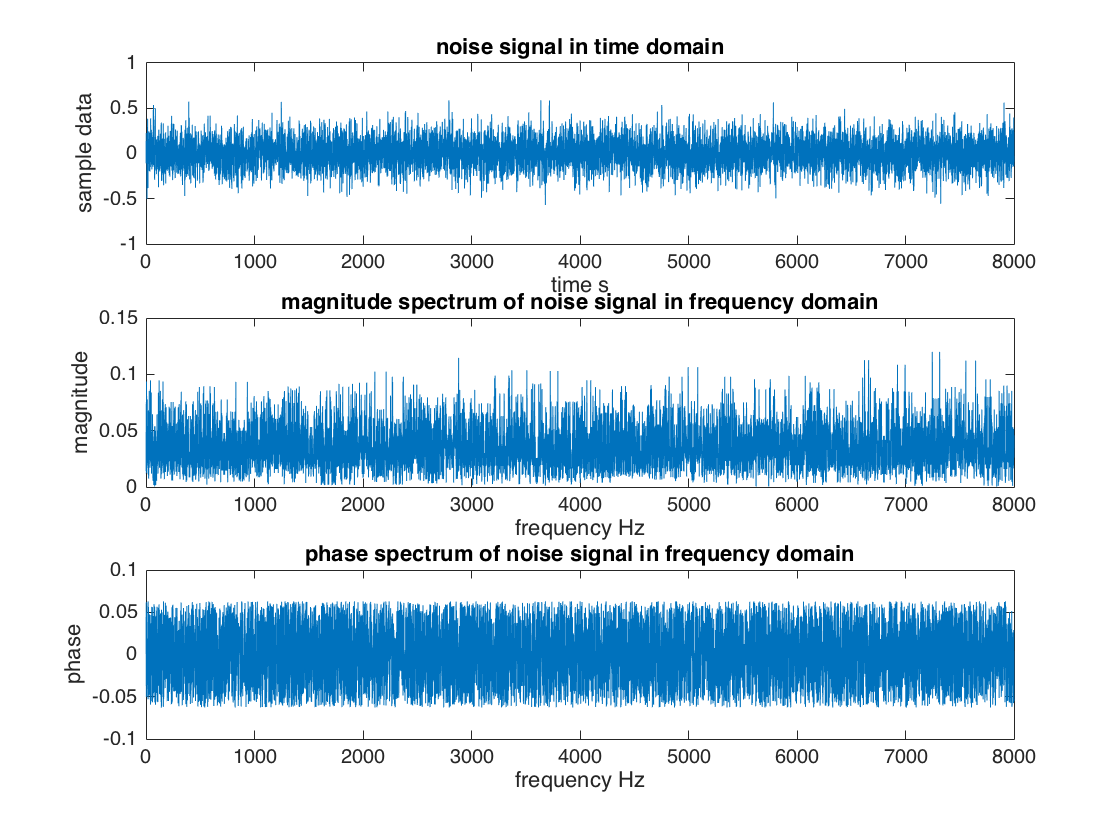
\includegraphics[width=3.5in]{fourier_transform_plot}
\begin{flushleft}
MATLAB function \textit{fft}, an implementation of fast Fourier transform, computes DFT in an efficient manner. On the other hand, function \textit{ifft}, an implementation of inverse fast Fourier transform, converts the signal from frequency domain back to time domain. With these two  functions, we can convert signals between their time and frequency domain representations.
\end{flushleft}

\subsection{Spectral Subtraction}
\begin{flushleft}
The spectral subtraction method is a simple and effective method of noise reduction. In this method, an average signal spectrum and average noise spectrum are estimated in parts of the recording and subtracted from each other, so that average signal-to-noise ratio (SNR) is improved. We can express spectral subtraction mathematically. Equation (1) is implemented for our first system:
\begin{equation}
|Y_\omega(\omega)| = max(|S_\omega(\omega)|-|N_\omega(\omega)|,0)
\end{equation}
Note, since the magnitude spectrum of a signal is the absolute value of the Fourier transform, it cannot be negative. So, any negative values resulting from the subtraction are set to 0. Below is an visualization of spectral subtraction using the formula. Clearly, the denoised signal is much cleaner than the original noisy signal. 
\end{flushleft}
\centering 
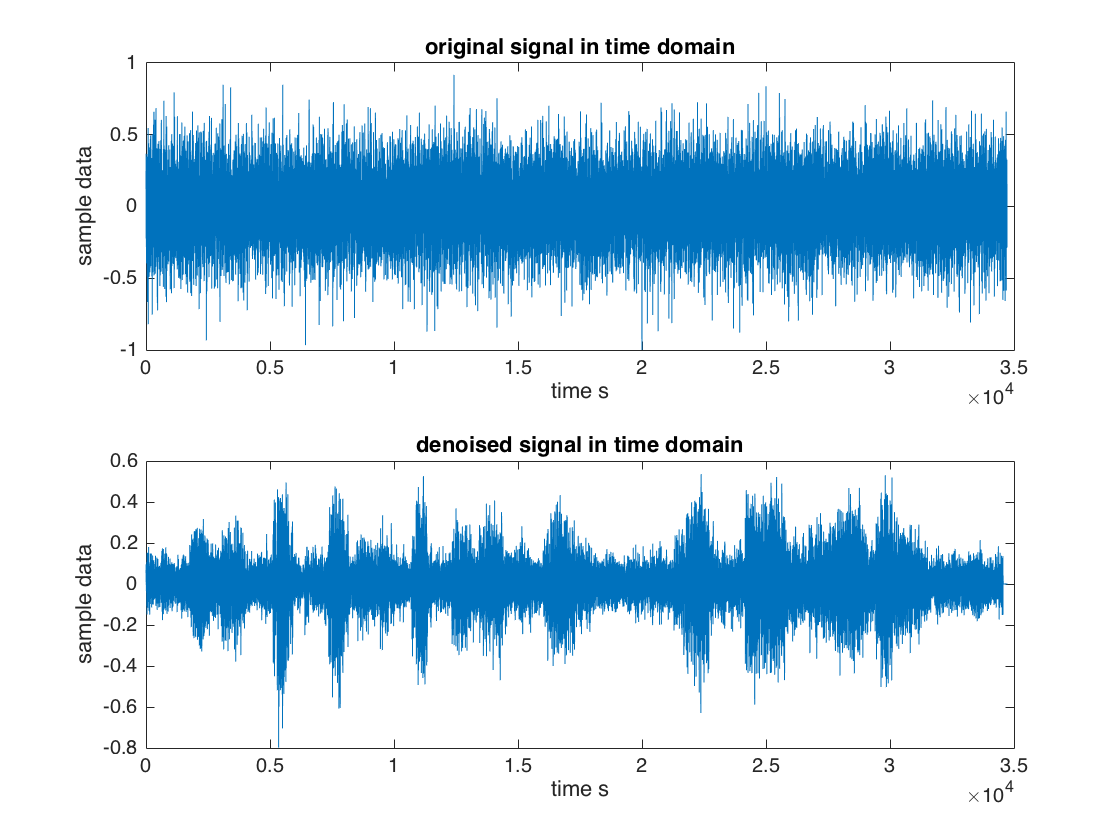
\includegraphics[width=3.5in]{spectral_subtraction_plot}

\begin{flushleft}
In our weighted noise cancellation system, we modify the first system by adding parameters $\alpha$ and $\beta$. The rationale behind this is to get rid of the whistling musical noise our first system generates by replacing the 0s with white noise $\beta|N_\omega(\omega)|$. By tweaking $\alpha$ and $\beta$, we can further improve the sound quality of the denoised signal. Equation 2 manifests the idea:
\begin{equation}
    |Y_\omega(\omega)| =
    \begin{cases}
      |S_\omega(\omega)|-\alpha|N_\omega(\omega)|, & \text{if}\ |S_\omega(\omega)| > |N_\omega(\omega)|\\
      \beta|N_\omega(\omega)|, & \text{otherwise}
    \end{cases}
\end{equation}
\end{flushleft}

\subsection{SNR}
\begin{flushleft}
Signal-to-noise ratio, abbreviated SNR, is a measure that compares the level of a desired signal to the level of background noise. It is defined as the ratio of signal power to the noise power. A ratio higher than 1:1 (greater than 0 dB) indicates more signal than noise. In our paper, SNR is an indicator of the noise level for each recordings. The formula of SNR is as followed:
\begin{equation}
SNR_\omega = 10\log_{10}(\frac{1}{T_\omega}\sum_{T_\omega} |y_\omega(t)|^2) - 10\log_{10}(\frac{1}{T_\omega}\sum_{T_\omega} |n_\omega(t)|^2)
\end{equation}
Theoretically, a higher SNR indicates better sound quality of the output signal. However, this is not the case in our weighted noise cancellation system, since we add white noise to the original signals to eliminate musical noise. A higher SNR in fact indicates a higher level of white noise. 
\end{flushleft}

% needed in second column of first page if using \IEEEpubid
%\IEEEpubidadjcol

% An example of a floating figure using the graphicx package.
% Note that \label must occur AFTER (or within) \caption.
% For figures, \caption should occur after the \includegraphics.
% Note that IEEEtran v1.7 and later has special internal code that
% is designed to preserve the operation of \label within \caption
% even when the captionsoff option is in effect. However, because
% of issues like this, it may be the safest practice to put all your
% \label just after \caption rather than within \caption{}.
%
% Reminder: the "draftcls" or "draftclsnofoot", not "draft", class
% option should be used if it is desired that the figures are to be
% displayed while in draft mode.
%
%\begin{figure}[!t]
%\centering
%\includegraphics[width=2.5in]{myfigure}
% where an .eps filename suffix will be assumed under latex, 
% and a .pdf suffix will be assumed for pdflatex; or what has been declared
% via \DeclareGraphicsExtensions.
%\caption{Simulation Results}
%\label{fig_sim}
%\end{figure}

% Note that IEEE typically puts floats only at the top, even when this
% results in a large percentage of a column being occupied by floats.


% An example of a double column floating figure using two subfigures.
% (The subfig.sty package must be loaded for this to work.)
% The subfigure \label commands are set within each subfloat command, the
% \label for the overall figure must come after \caption.
% \hfil must be used as a separator to get equal spacing.
% The subfigure.sty package works much the same way, except \subfigure is
% used instead of \subfloat.
%
%\begin{figure*}[!t]
%\centerline{\subfloat[Case I]\includegraphics[width=2.5in]{subfigcase1}%
%\label{fig_first_case}}
%\hfil
%\subfloat[Case II]{\includegraphics[width=2.5in]{subfigcase2}%
%\label{fig_second_case}}}
%\caption{Simulation results}
%\label{fig_sim}
%\end{figure*}
%
% Note that often IEEE papers with subfigures do not employ subfigure
% captions (using the optional argument to \subfloat), but instead will
% reference/describe all of them (a), (b), etc., within the main caption.


% An example of a floating table. Note that, for IEEE style tables, the 
% \caption command should come BEFORE the table. Table text will default to
% \footnotesize as IEEE normally uses this smaller font for tables.
% The \label must come after \caption as always.
%
%\begin{table}[!t]
%% increase table row spacing, adjust to taste
%\renewcommand{\arraystretch}{1.3}
% if using array.sty, it might be a good idea to tweak the value of
% \extrarowheight as needed to properly center the text within the cells
%\caption{An Example of a Table}
%\label{table_example}
%\centering
%% Some packages, such as MDW tools, offer better commands for making tables
%% than the plain LaTeX2e tabular which is used here.
%\begin{tabular}{|c||c|}
%\hline
%One & Two\\
%\hline
%Three & Four\\
%\hline
%\end{tabular}
%\end{table}


% Note that IEEE does not put floats in the very first column - or typically
% anywhere on the first page for that matter. Also, in-text middle ("here")
% positioning is not used. Most IEEE journals use top floats exclusively.
% Note that, LaTeX2e, unlike IEEE journals, places footnotes above bottom
% floats. This can be corrected via the \fnbelowfloat command of the
% stfloats package.


\section{Noise Cancellation System}
\begin{flushleft}
In this section, we implement our first noise cancellation with Equation (1) and inspect the effect of window size $T_\omega$ have on the sound quality. 
\end{flushleft}

\subsection{Implementation}
\begin{flushleft}
Sample the \textit{.wav} files with MATLAB function \textit{audioread}, and store the sampling data in a 2D matrix $x_\omega$. We also pad $x_\omega$ with 0s at the end. Number of data per frame \textit{frame} is $\frac{Tms*Fs}{1000}$. In the current project, we assume that the first 1 second of each recording has no speech content. Hence the number of noise frames \textit{nFrame} is $\frac{1*1000}{Tms}$ and the number of speech frames \textit{sFrame} is $\frac{length(x_\omega)}{\textit{frame}} - \textit{nFrames}$. We then loop over $x_\omega$ and store the noise portion at $n_\omega$ and the speech portion at $s_\omega$, which are both 2D matrices. 
\end{flushleft}

\begin{flushleft}
Noise estimation is done by looping over each frame of $n_\omega$, taking the fast Fourier transform with \textit{fft} for each frame, and taking the average over all frames. We store the resulting cell array at $N_\omega$. Note that we also specify the Fourier transform coefficient \textit{FFT-coeff} to 160. This allows us to lower the feature dimension and improve the overall sound quality.
\end{flushleft}

\begin{flushleft}
To construct the denoised signal, we use spectrum subtraction by implementing Equation (1). Take a window of same size as the frame, slide through $s_\omega$, and take the Fourier transform of the window. The denoised signal in the frequency domain can be computed with Equation (4): 
\begin{equation}
Y_\omega(\omega) = |Y_\omega(\omega)|e^{j\angle S_\omega(\omega)}
\end{equation}
We then take the inverse fast Fourier transform of it with \textit{ifft} to convert it back to time domain, and store it in a cell array \textit{y1}. A visualization of white noise sample 15 with time frame 20ms is at below. Clearly, the signal is much cleaner after the noise cancellation.
\end{flushleft}
\centering 
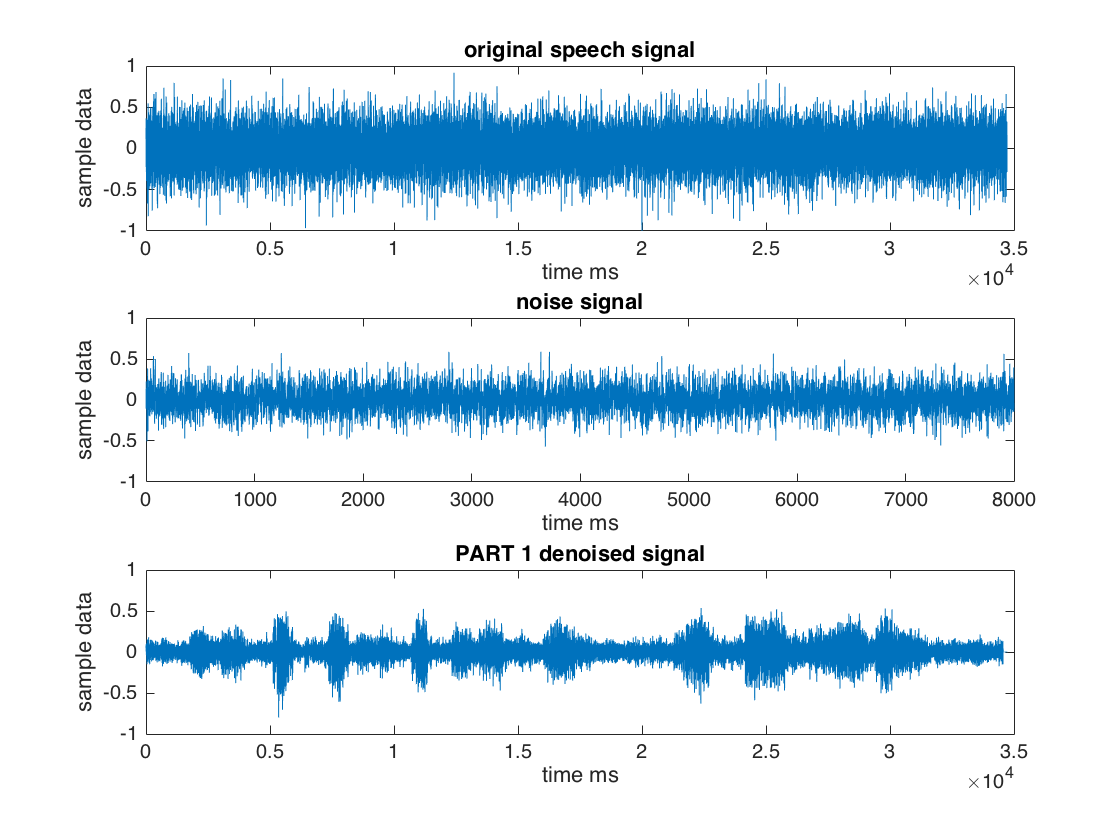
\includegraphics[width=3.5in]{plot1}

\subsection{Effect of $T_\omega$}
\begin{flushleft}
We experiment different time frames $T_\omega$ (i.e. window size) and the effect they have. Below are three plots with $T_\omega = 20ms$, $T_\omega = 100ms$, and $T_\omega = 500ms$. As we can see, $T_\omega = 20ms$'s plot is much denser and much more data points. The sound quality also proves that $T_\omega = 20ms$ has much better quality than the other two. After experimenting different frame sizes, we find $T_\omega = 20ms$ has generally the best quality for all recordings. 
\end{flushleft}
\centering 
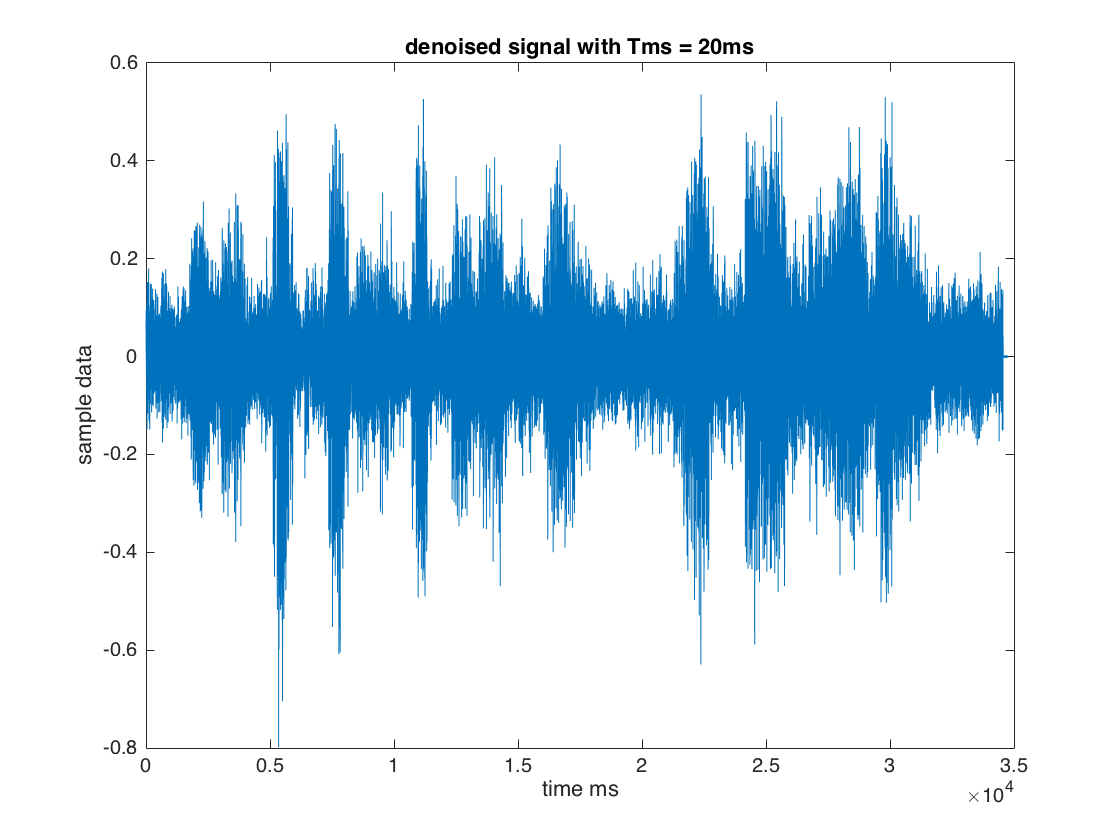
\includegraphics[width=2in]{20ms}
\centering 
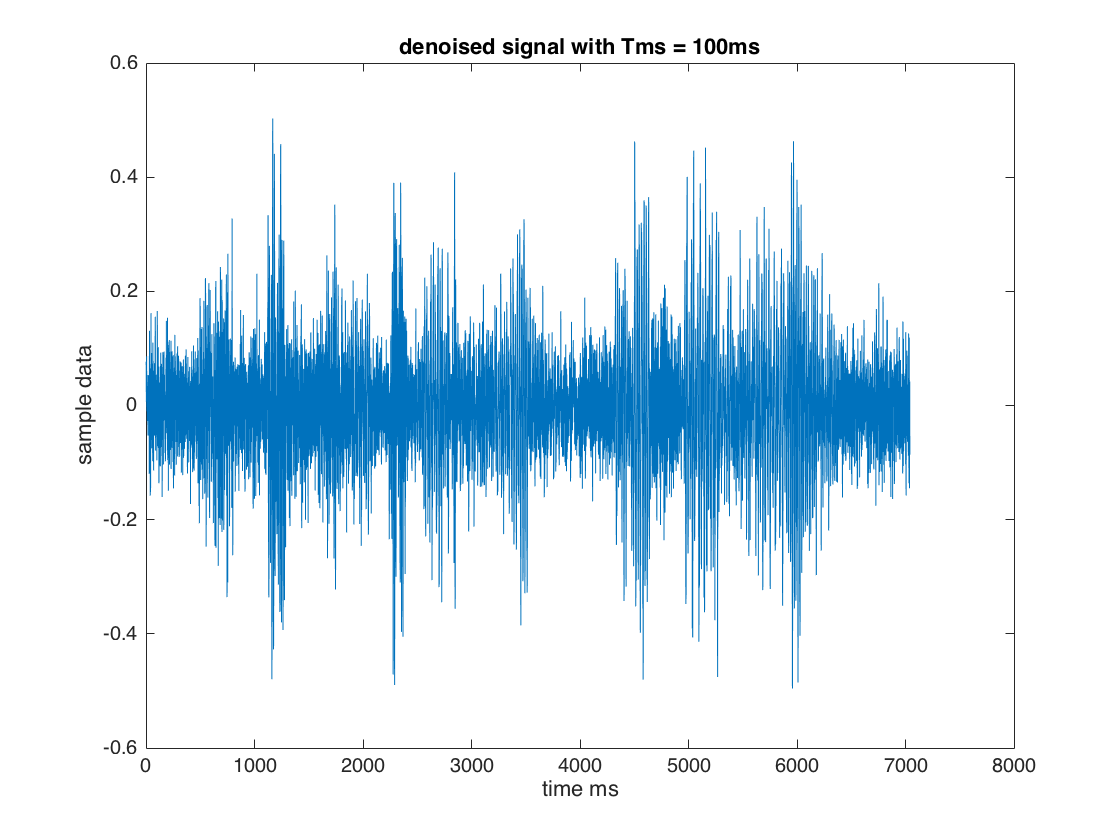
\includegraphics[width=2in]{100ms}
\centering 
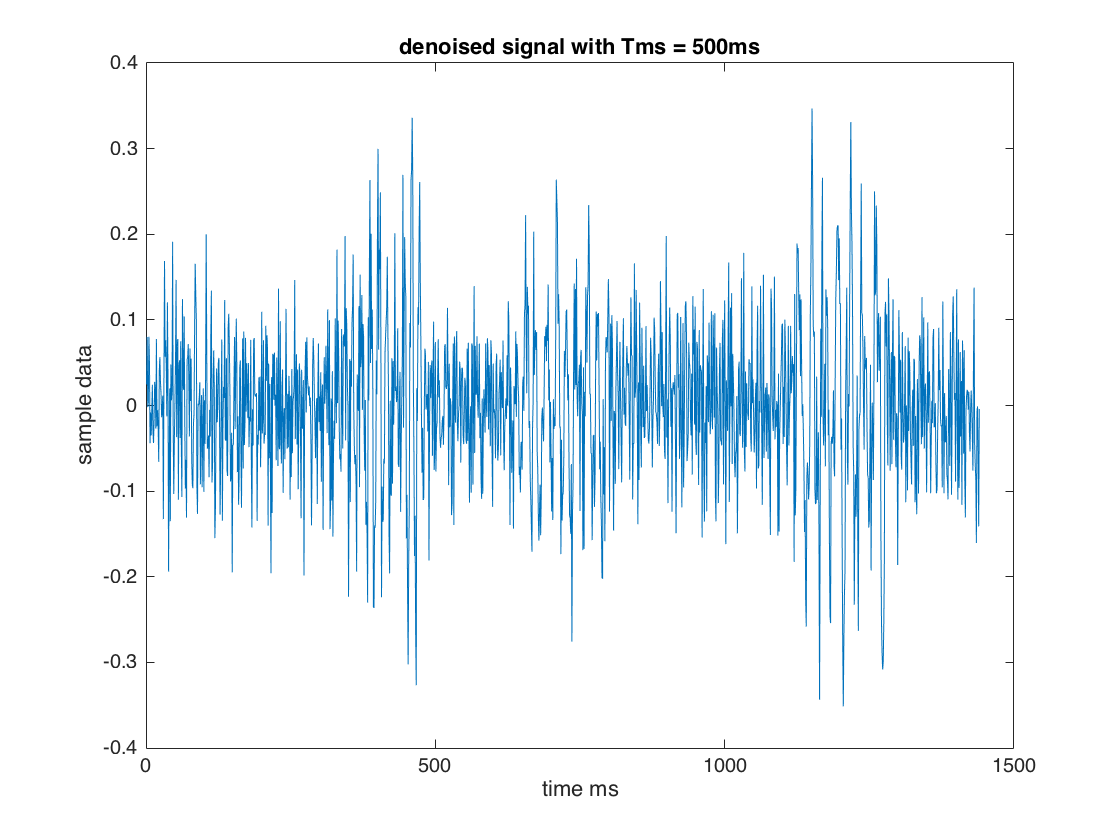
\includegraphics[width=2in]{500ms}

\section{Weighted Noise Cancellation System}
\begin{flushleft}
In this section, we aim to modify our first noise cancellation with Equation (2) and eliminate the whistling musical noise. We also inspect the effect of $\alpha$ and $\beta$ have on the sound quality as well as the correlation between SNR, $\alpha$ and $\beta$.
\end{flushleft}
\subsection{Equation (2) Implementation}
\begin{flushleft}
Intuitively speaking, Equation (2) allows us to control how much noise to subtract ($\alpha$) and to leave ($\beta$) in the signal. Replacing 0s with $\beta|N_\omega(\omega)|$ get rid of musical noise, yet this also adds white noise to the reconstructed signal. 
\end{flushleft}

\begin{flushleft}
Implementations of Equation (1) and Equation (2) are similar. Take a window of same size as the frame, slide through $s_\omega$, and take the Fourier transform of the window with the same Fourier coefficient \textit{FFT-coeff} as the nosie estimation. However, before advancing the window to the next frame, we compare every data point in the frame with the corresponding data point in $N_\omega(\omega)$, and with Equation (4) we make decision of the new reconstructed signal, storing it in a cell array \textit{recons-freq}. Now, we can compute the denoised signal in the frequency domain can be computed with Equation (4), and restore it to time domain with \textit{ifft}, storing it in a cell array \textit{y2}. Note that in the \textit{ifft} operation, we only take the real part out of it for the time domain. Hence, we lose some information from the complex domain. A visualization of the weighted noise cancellation system with white noise signal 1, $\alpha = 2.8$, $\beta = 0.8$ is as follows. 
\end{flushleft}
\centering 
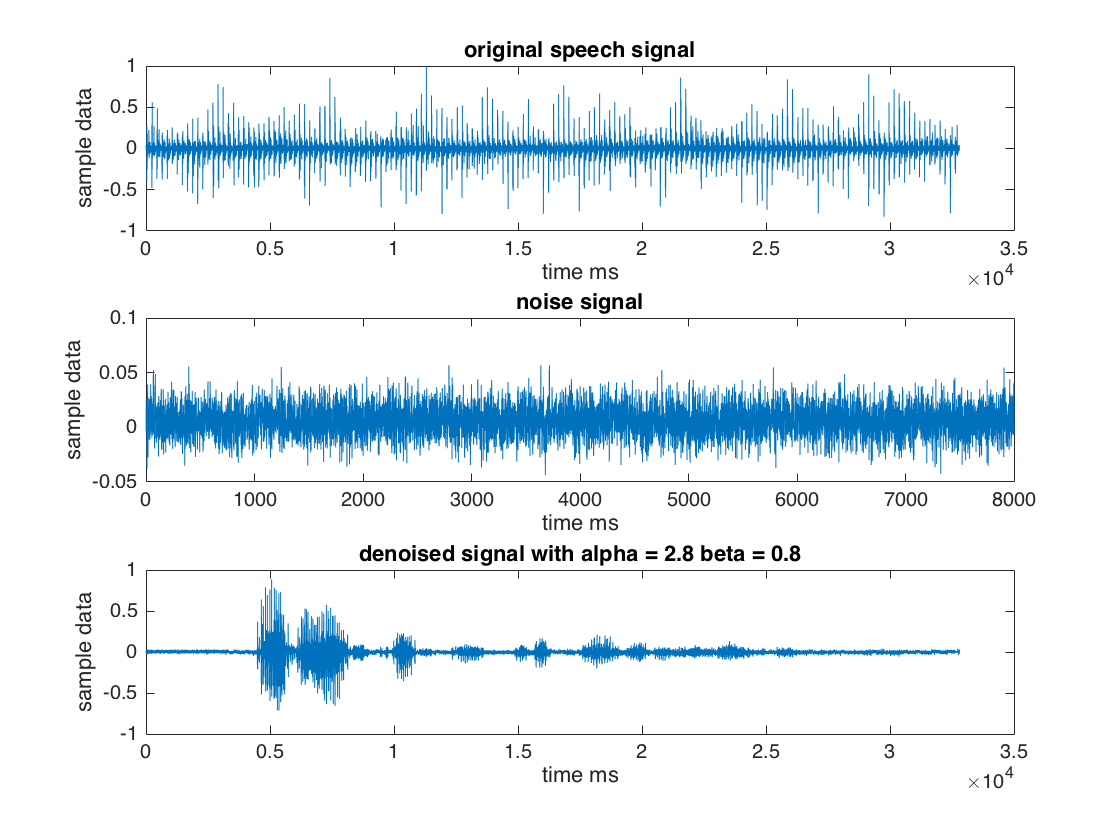
\includegraphics[width=3.5in]{plot2}

\begin{flushleft}
A comparison between the two noise cancellation systems is at below. As one can see, the two output signals look very similar, yet the signal generated by the weighted noise cancellation system has much better sound quality. The musical noise disappears with little white noise added to it. 
\end{flushleft}
\centering 
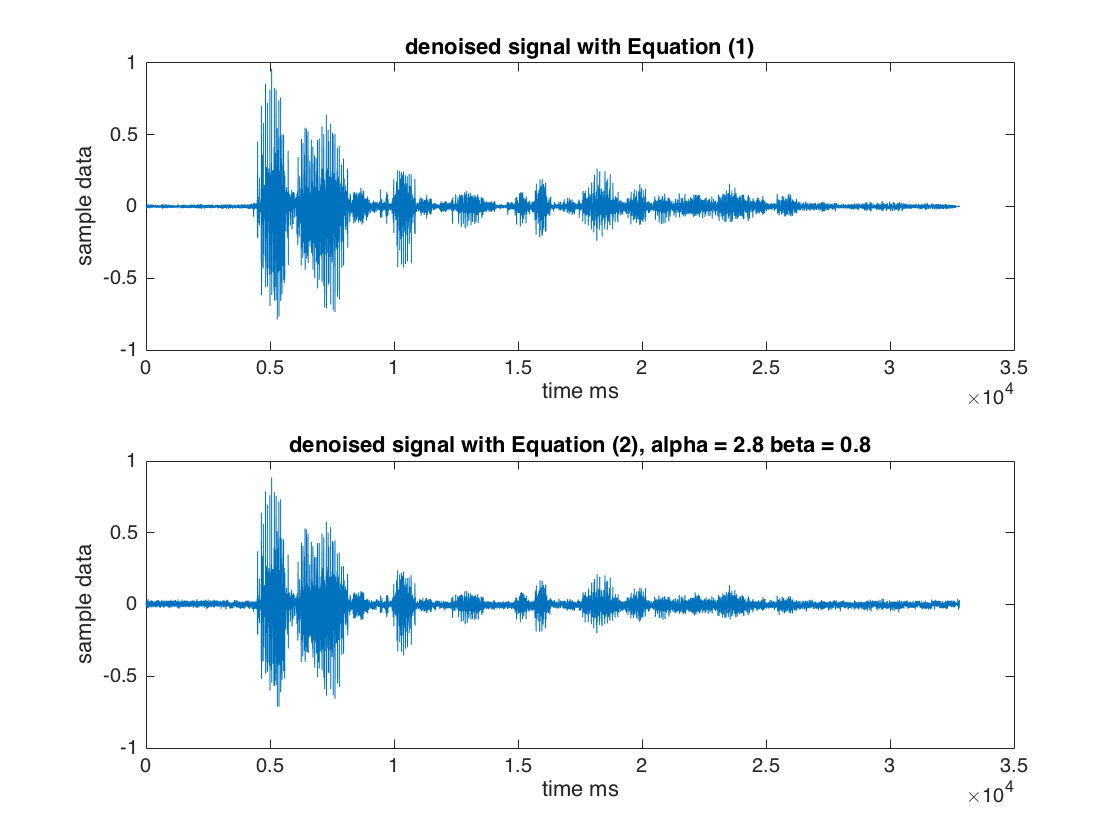
\includegraphics[width=3.5in]{plot3}

\subsection{SNR Implementation}
\begin{flushleft}
Equation (3)'s implementation is straightforward. Compute the noise power estimation $10\log_{10}(\frac{1}{T_\omega}\sum_{T_\omega} |n_\omega(t)|^2)$ of the signal first. We call it \textit{noise-est}. To achieve this, loop over every frame of $n_\omega$, and with MATLAB function \textit{sum} and \textit{power} we can compute noise power estimation for one frame. Noise power estimation for the entire signal is averaging noise power estimation of every frame. 
\end{flushleft}

\begin{flushleft}
The rest of Equation (3) follows a similar manner. Loop over every frame of $s_\omega$, compute the signal power estimation for every frame and subtracts it with \textit{noise-est}. Store these values in a cell array \textit{SNR1}, and with MATLAB function \textit{mean}, we obtain the average SNR for the signal. 
\end{flushleft}

\subsection{Choice of $\alpha$ and $\beta$}
\begin{flushleft}
After testing out different sets of $\alpha$ and $\beta$ on the white noise dataset, $\alpha = 2.8$ and $\beta = 0.8$ outperforms the other combinations. 
\end{flushleft}
  
\begin{flushleft}
To understand the effect of $\alpha$, we set $\beta = 0.8$ and visualize $\alpha = 1$, $\alpha = 5$ and $\alpha = 10$ ($T_\omega = 20ms$ with white noise signal 10). We find out that the higher the $\alpha$ value is, the more unclear the actual speech is. This indicates an inversely proportional relationship between the $\alpha$ value and SNR. 
\end{flushleft}
\centering 
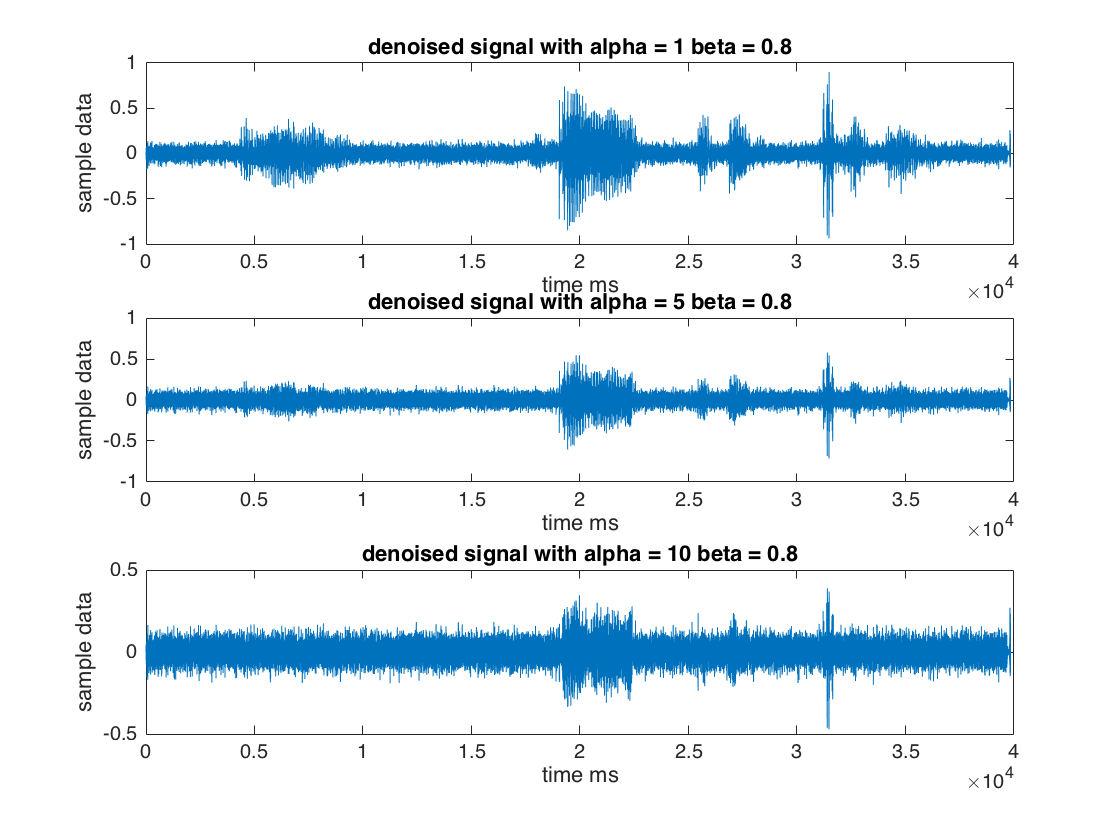
\includegraphics[width=3.5in]{alpha1}

\begin{flushleft}
On the other hand, to understand the effect of $\beta$, we set $\alpha = 2.8$ and visualize $\beta = 0.1$, $\beta = 0.5$ and $\beta = 0.1$ ($T_\omega = 20ms$ with white noise signal 8). We find out that the higher the $\beta$ value is, the nosier the actual speech is (i.e. more white noise). However, the $\beta$ value is surprisingly proportional to SNR. The phenomena can be understood by Equation (2). When we increase $\beta$, both power levels of the reconstructed and noise signal increase, resulting in an increase in SNR. Hence, SNR may not be a good indicator of choosing $\alpha$ and $\beta$. Note, $\beta$ is between 0 and 1 since we do not want reconstructed signal has higher noise level than its original signal.  
\end{flushleft}
\centering 
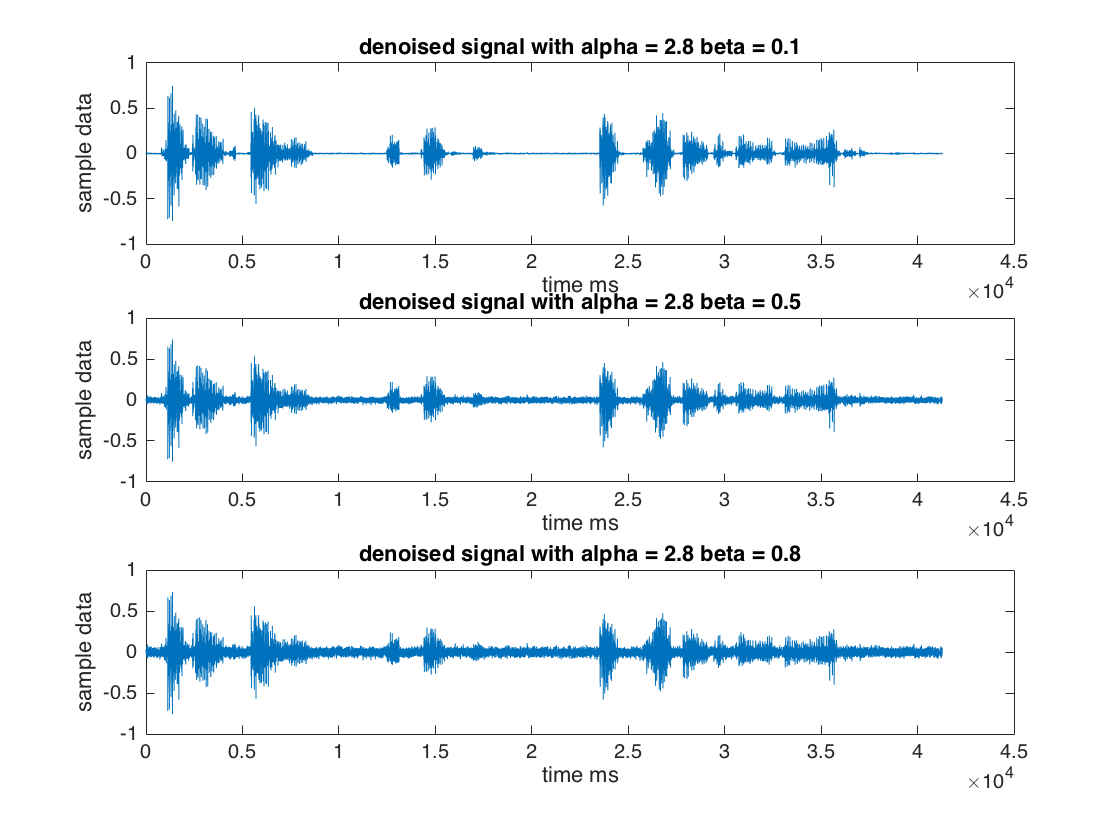
\includegraphics[width=3.5in]{alpha2}

\section{Effect of Noise}
\begin{flushleft}
In this section, we examine how different noise types corrupt a speech signal. We will discuss how different noise affects a signal, and which $\alpha$, $\beta$, and $T_\omega$ work best in each case. 
\end{flushleft}

\subsection{White noise}
\begin{flushleft}
White noise is a random signal having equal intensity at different frequencies, giving it a constant power spectral density. It is not as high pitch as violet noise nor as low pitch as pink noise. A frequency spectrum of white noise is generated below ($\alpha = 2.8$, $\beta = 0.8$, $T_\omega = 20ms$). As one can see, the power density is about uniform for every frequency.
\end{flushleft}
\centering 
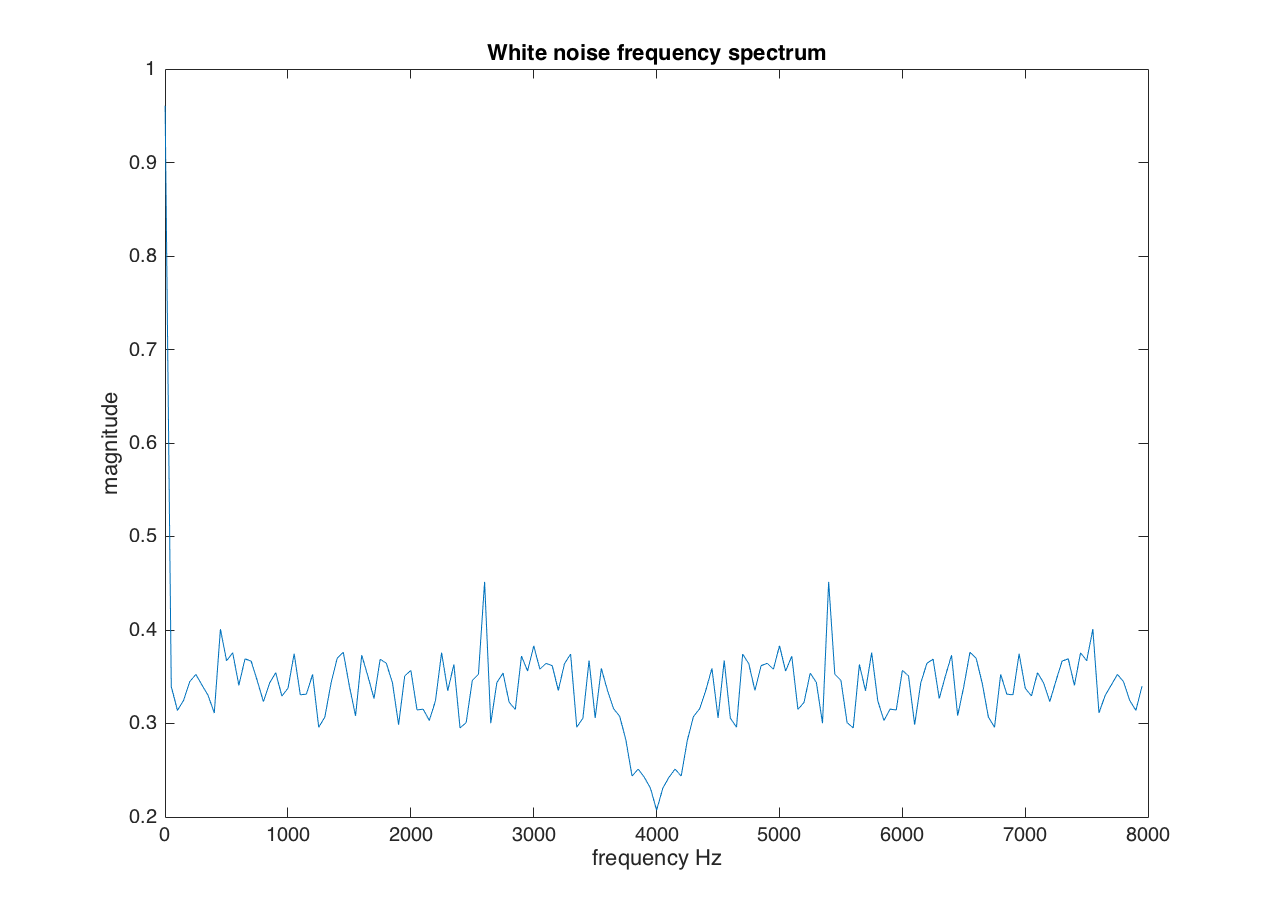
\includegraphics[width=3.5in]{whitenoise_log}
\begin{flushleft}
The combination of $\alpha = 2.8$, $\beta = 0.8$, and $T_\omega = 20ms$ work best for white noise. $T_\omega = 20ms$ plays the reconstructed signal at a desired speed, $\beta = 0.8$ gives the signal a desired amount of white noise, and $\alpha = 2.8$ subtract majority of the noise from speech. Visualization of such combination is as followed. 
\end{flushleft}
\centering 
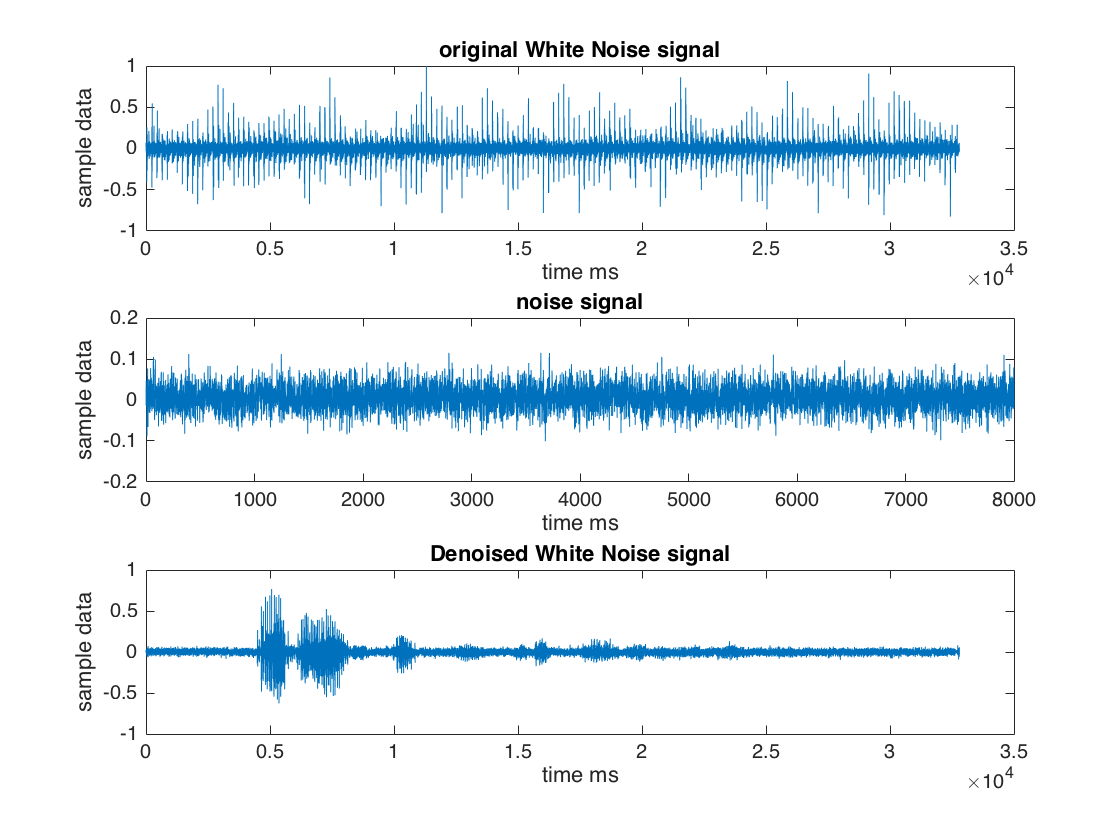
\includegraphics[width=3.5in]{WhiteNoise}

\subsection{Violet noise}
\begin{flushleft}
Violet noise is a signal with a frequency spectrum such that the spectral energy density is proportional to the frequency squared. It has the highest pitch among the five noises. A frequency spectrum of violet noise is generated below ($\alpha = 2.8$, $\beta = 0.8$, $T_\omega = 20ms$). As one can see, the power level is much higher at high frequencies.
\end{flushleft}
\centering 
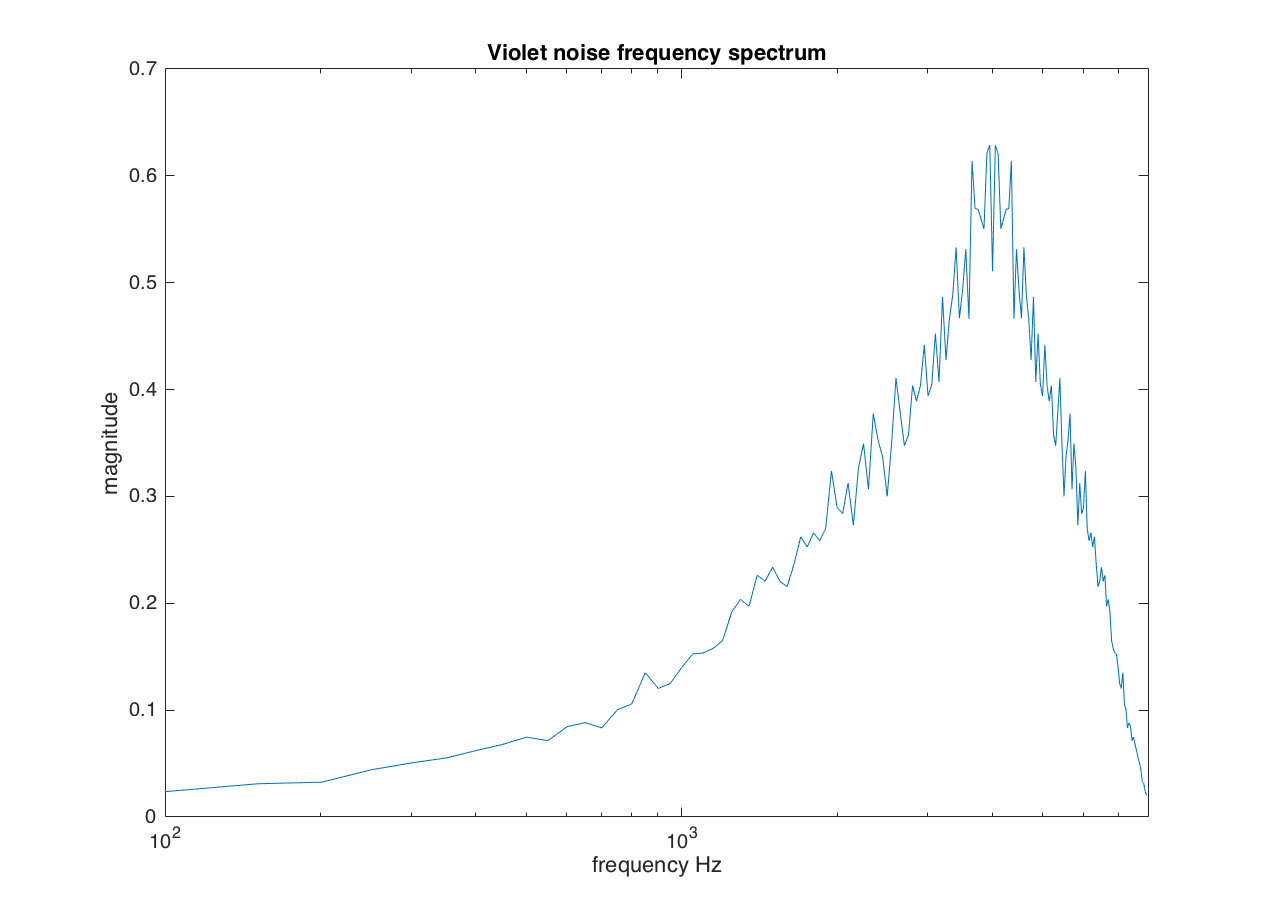
\includegraphics[width=3.5in]{violetnoise_log}
\begin{flushleft}
The combination of $\alpha = 2.5$, $\beta = 0.5$, and $T_\omega = 20ms$ work best for violet noise. $T_\omega = 20ms$ plays the reconstructed signal at a desired speed, $\beta = 0.5$ gives the signal a desired amount of noise, and $\alpha = 2.5$ subtract majority of violet noise from speech. Visualization of such combination is as followed. 
\end{flushleft}
\centering 
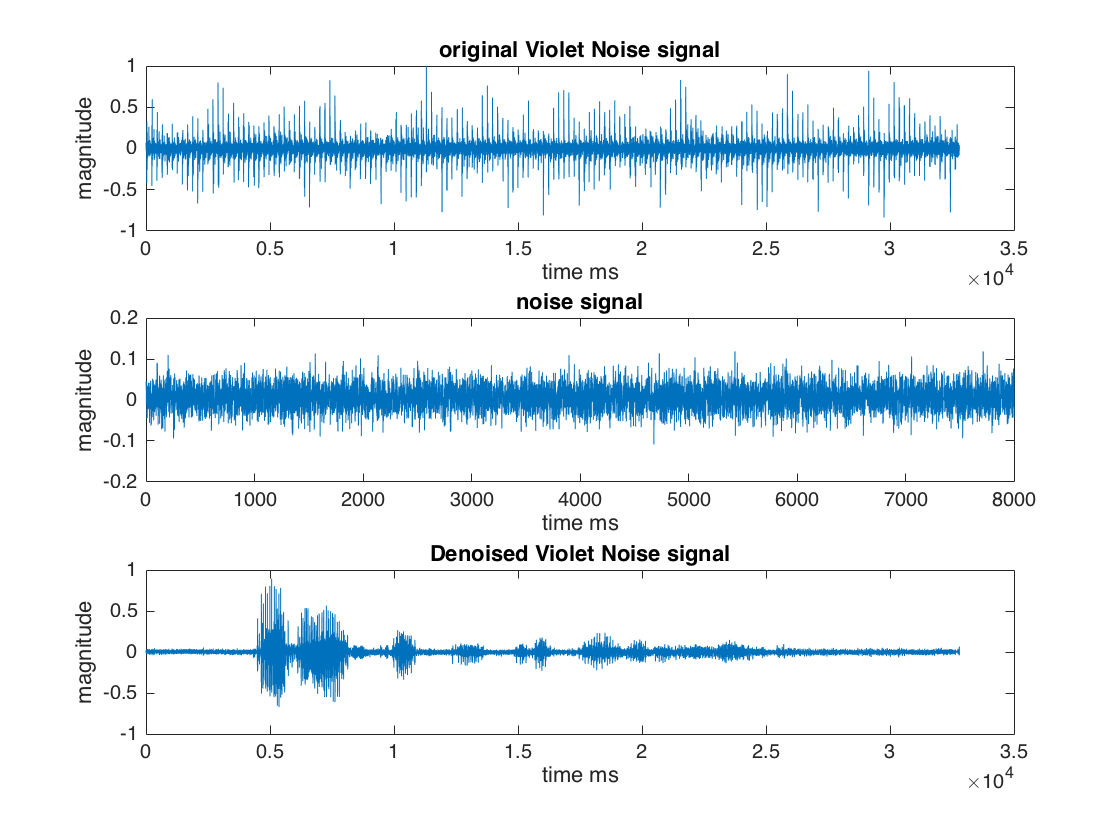
\includegraphics[width=3.5in]{violetNoise}

\subsection{Pink noise}
\begin{flushleft}
Pink noise is a signal with a frequency spectrum such that the power spectral density (energy or power per frequency interval) is inversely proportional to the frequency of the signal. It has the lowest pitch among the five noises. A frequency spectrum of pink noise is generated below ($\alpha = 2.8$, $\beta = 0.8$, $T_\omega = 20ms$). As one can see, the power level is much higher at low frequencies.
\end{flushleft}
\centering 
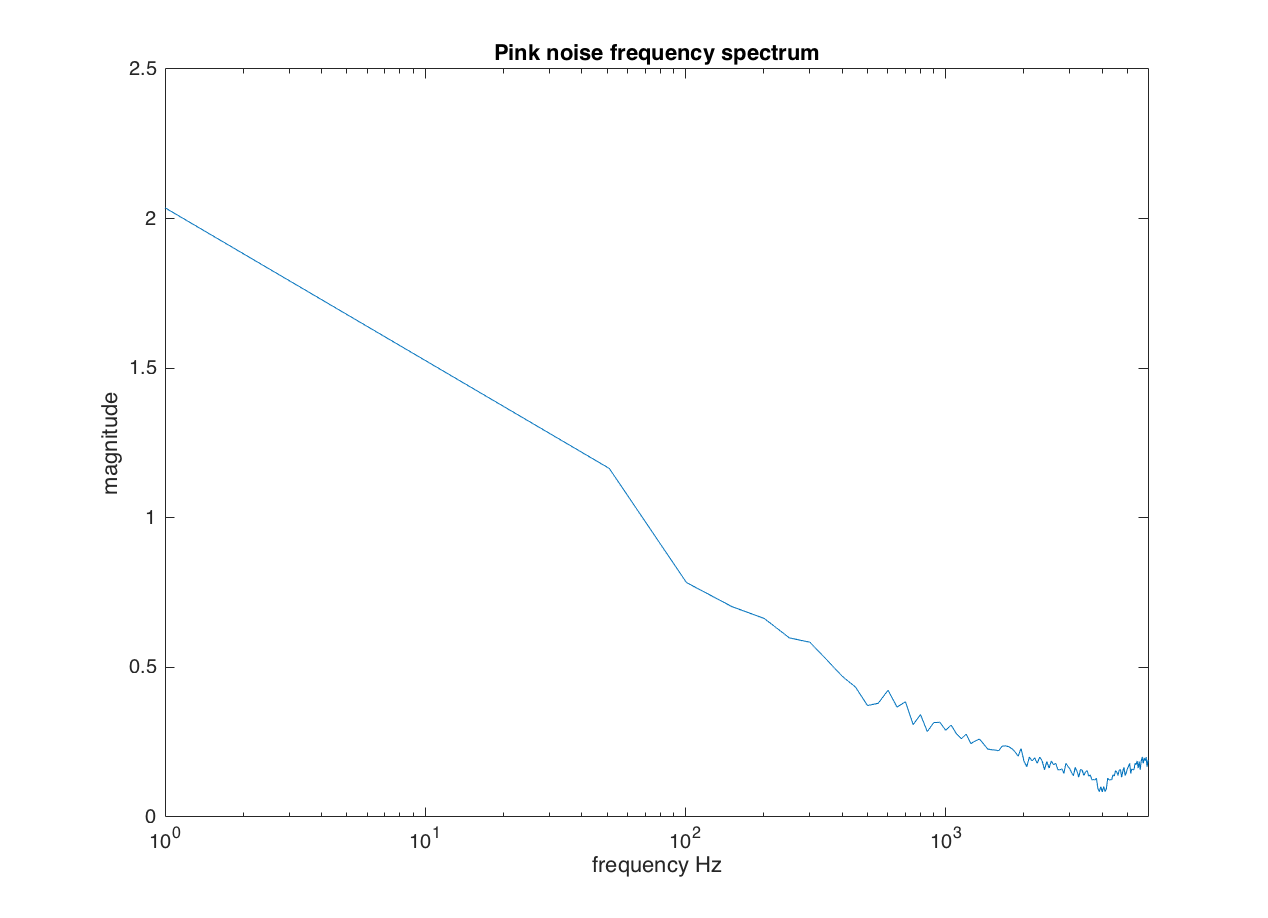
\includegraphics[width=3.5in]{pinknoise_log}
\begin{flushleft}
The combination of $\alpha = 1.8$, $\beta = 0.5$, and $T_\omega = 20ms$ work best for pink noise. $T_\omega = 20ms$ plays the reconstructed signal at a desired speed, $\beta = 0.5$ gives the signal a desired amount of noise, and $\alpha = 1.8$ subtract majority of pink noise from speech. Visualization of such combination is as followed. 
\end{flushleft}
\centering 
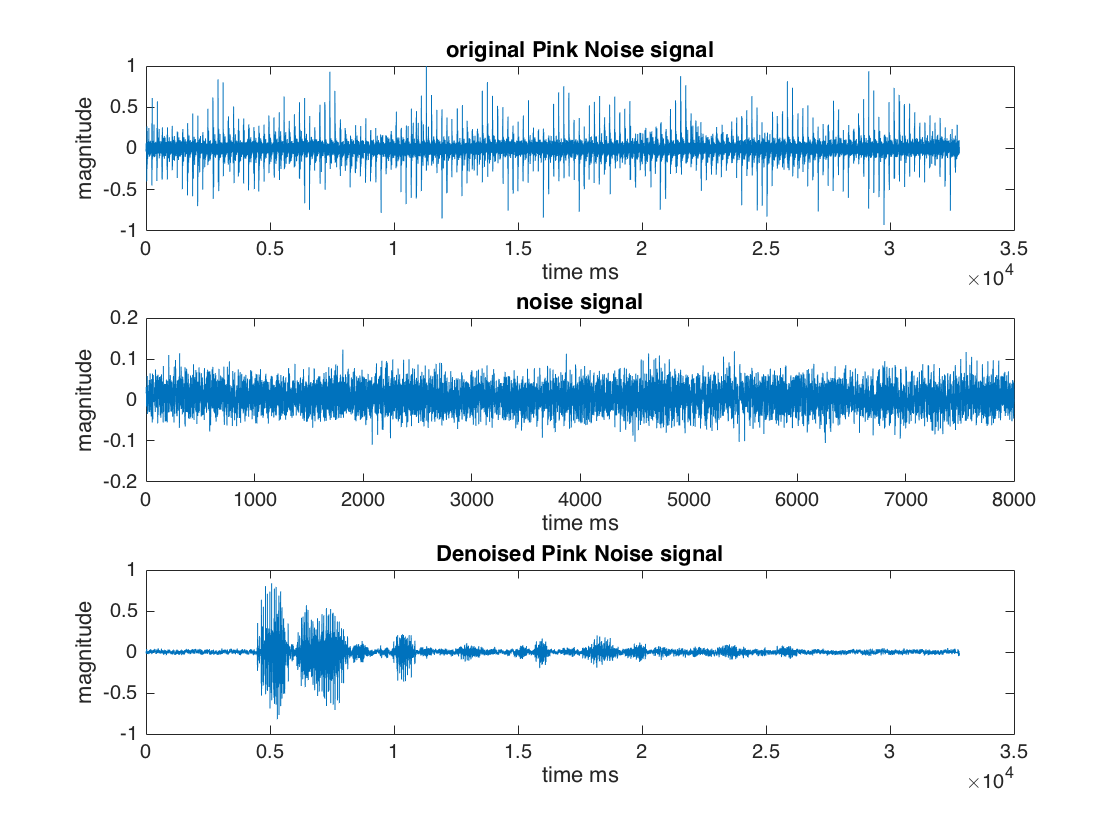
\includegraphics[width=3.5in]{pinkNoise}

\subsection{Grey noise}
\begin{flushleft}
Grey noise is a random noise whose frequency spectrum follows a psychoacoustic equal loudness curve. Comparing to white noise, which contains all fequencies with eqaul energy, grey noise contains all frequencies with equal loudness. It has the smallest and most stable amplitude out of the five noises. A frequency spectrum of grey noise is generated below ($\alpha = 2.8$, $\beta = 0.8$, $T_\omega = 20ms$). As one can see, the power level is low and stable for all frequencies.
\end{flushleft}
\centering 
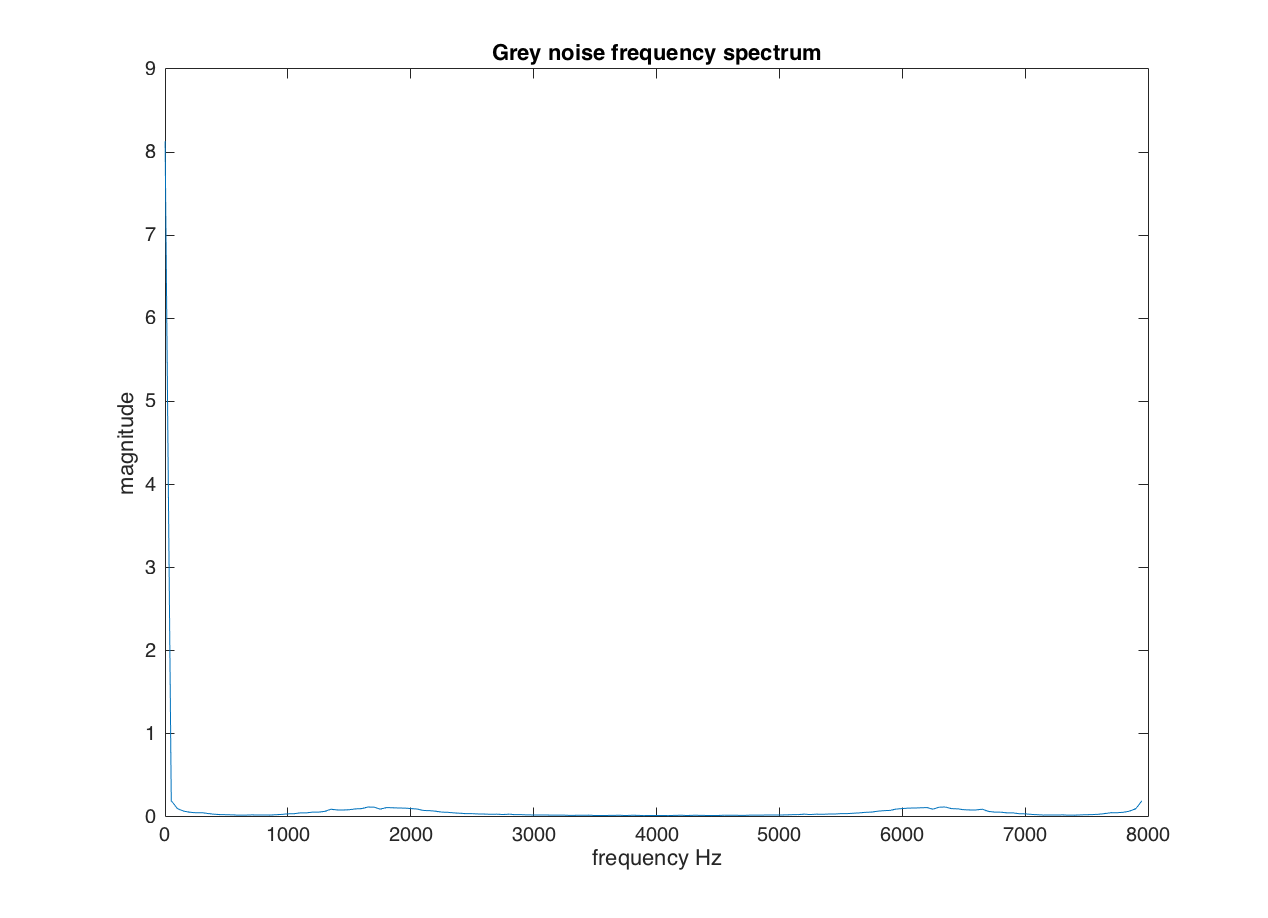
\includegraphics[width=3.5in]{greynoise_log}
\begin{flushleft}
The combination of $\alpha = 1.5$, $\beta = 0.5$, and $T_\omega = 20ms$ work best for grey noise. $T_\omega = 20ms$ plays the reconstructed signal at a desired speed, $\beta = 0.5$ gives the signal a desired amount of noise, and $\alpha = 1.5$ subtract majority of grey noise from speech. Visualization of such combination is as followed. 
\end{flushleft}
\centering 
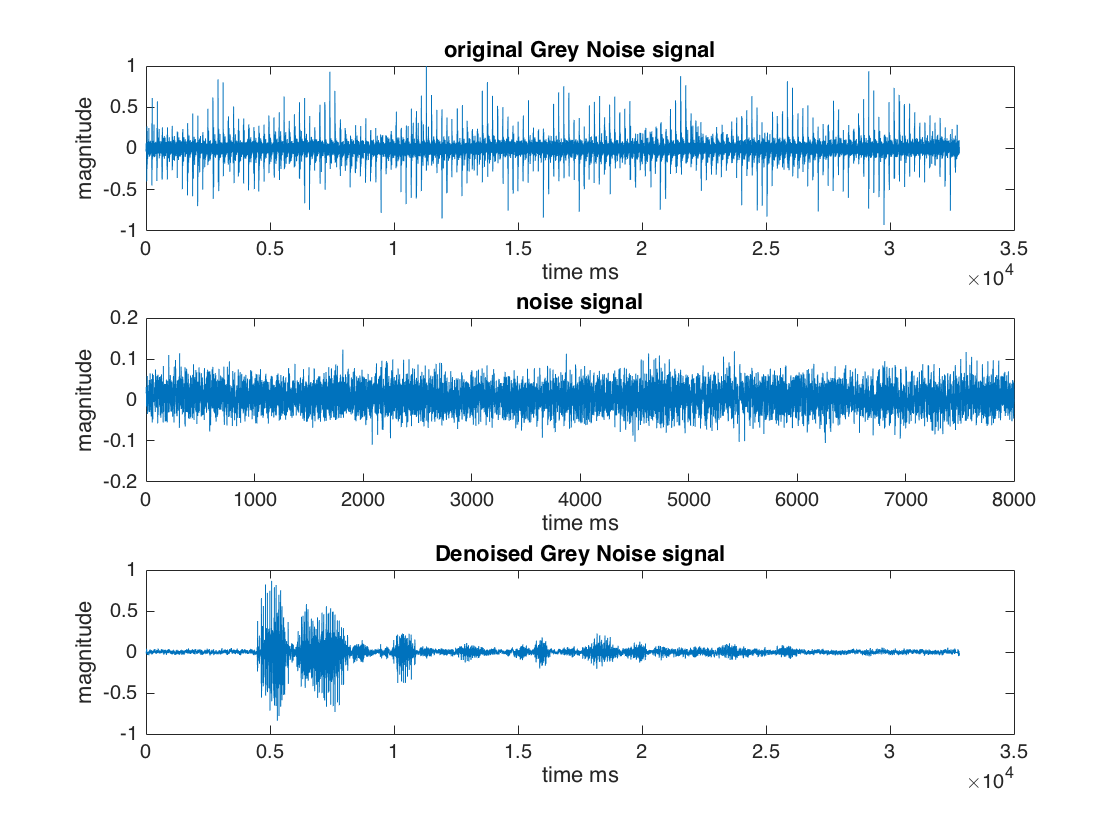
\includegraphics[width=3.5in]{greyNoise}

\subsection{f16 noise}
\begin{flushleft}
f16 noise is a random noise very similar to white noise. A frequency spectrum of f16 noise is generated below ($\alpha = 2.8$, $\beta = 0.8$, $T_\omega = 20ms$). As one can see, there is not really a noise pattern, since the jet noise is recorded from the environment. 
\end{flushleft}
\centering 
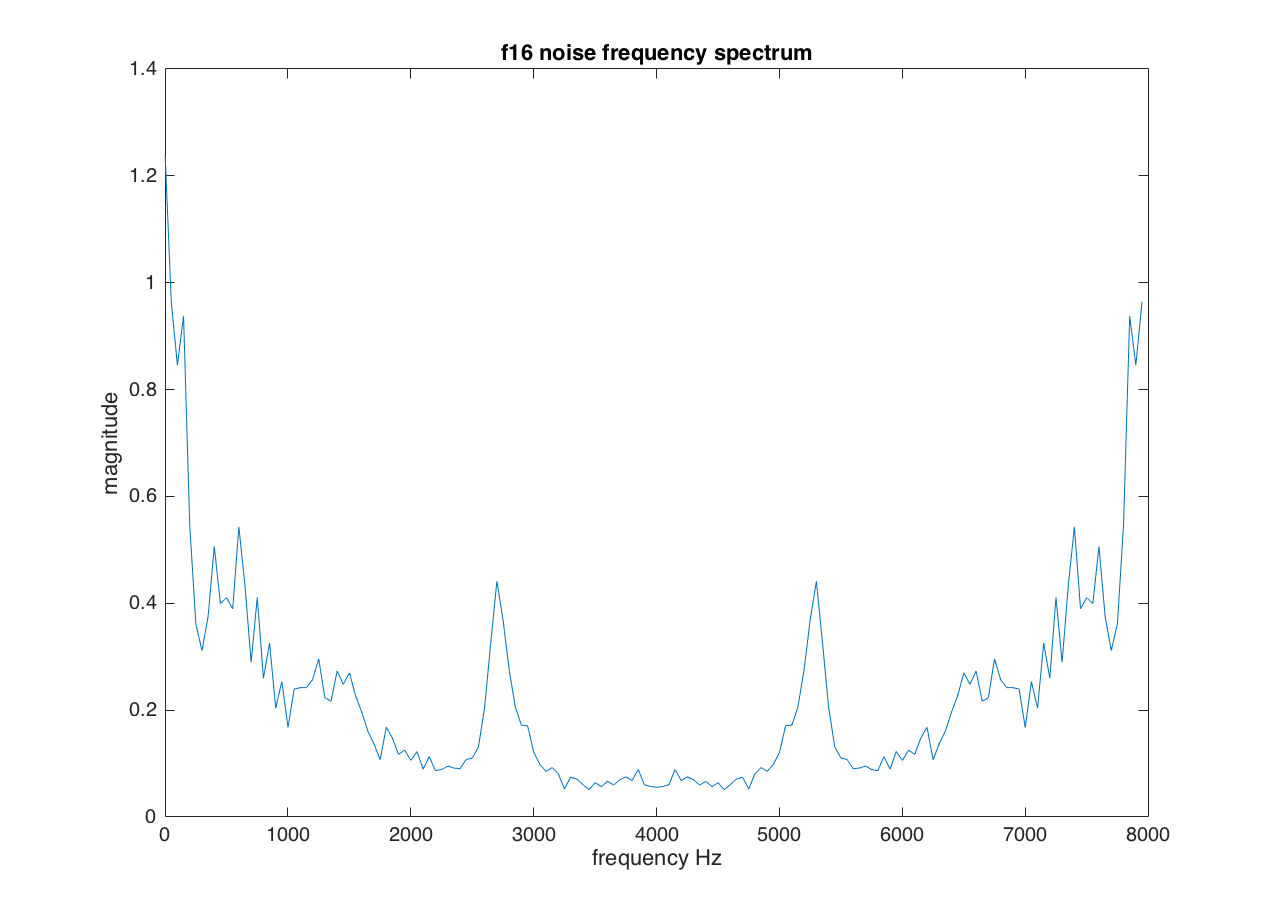
\includegraphics[width=3.5in]{f16noise_log}
\begin{flushleft}
The combination of $\alpha = 2.1$, $\beta = 0.6$, and $T_\omega = 20ms$ work best for f16 noise. $T_\omega = 20ms$ plays the reconstructed signal at a desired speed, $\beta = 0.6$ gives the signal a desired amount of noise, and $\alpha = 2.1$ subtract majority of f16 noise from speech. Visualization of such combination is as followed. 
\end{flushleft}
\centering 
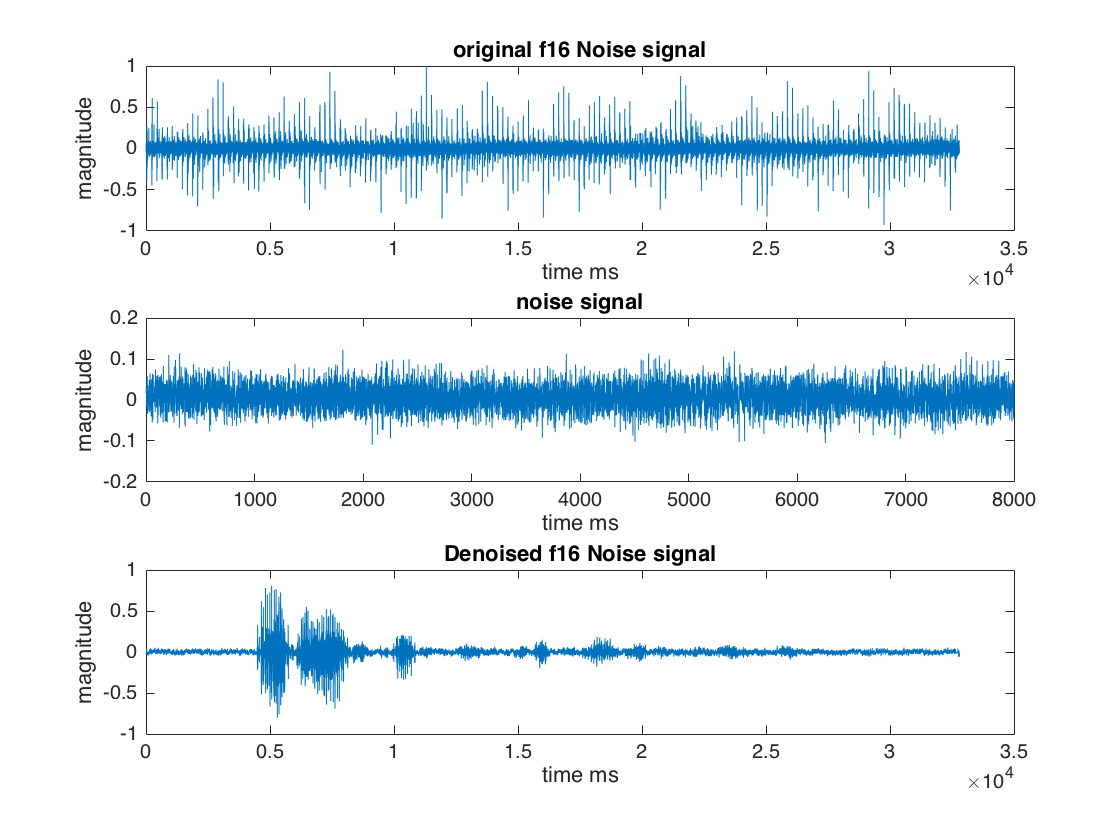
\includegraphics[width=3.5in]{f16Noise}

\subsection{Comparison}
\begin{flushleft}
The factors selection process can not be automate with the information given at the moment, even with machine learning algorithms. However, adding factor such as fundamental frequency can further assist the selection process and output better sound quality. Looking at the frequency spectrum of violet noise and pink noise, their power level has distinct difference between low and high frequencies. Therefore, we reasonably deduce factors should not be fixed for violet and pink noise. On the other hand, white, grey and f16 noise has stable power level. Changing factors over time will not make significant difference. 
\end{flushleft}

\section{Conclusion}
\begin{flushleft}
In this paper, we implement two noise cancellation systems and evaluate them on different kinds of noise. Detailed analysis on effects of $\alpha$ and $\beta$ on SNR along with visualizations are included. Future improvements include updating noise estimation for every frame in the entire signal and automate factors $\alpha$ and $\beta$ selection process by exploring new factors and implementing machine learning algorithms. Overall, this paper gives a general overview of the basic techniques and general flow of the experimental setup of noise cancellation system. 
\end{flushleft}

% if have a single appendix:
%\appendix[Proof of the Zonklar Equations]
% or
%\appendix  % for no appendix heading
% do not use \section anymore after \appendix, only \section*
% is possibly needed

% use appendices with more than one appendix
% then use \section to start each appendix
% you must declare a \section before using any
% \subsection or using \label (\appendices by itself
% starts a section numbered zero.)
%


% \appendices
% \section{Proof of the First Zonklar Equation}
% Some text for the appendix.

% use section* for acknowledgement
% \section*{Acknowledgment}


% The authors would like to thank...


% Can use something like this to put references on a page
% by themselves when using endfloat and the captionsoff option.
% \ifCLASSOPTIONcaptionsoff
%   \newpage
% \fi



% trigger a \newpage just before the given reference
% number - used to balance the columns on the last page
% adjust value as needed - may need to be readjusted if
% the document is modified later
%\IEEEtriggeratref{8}
% The "triggered" command can be changed if desired:
%\IEEEtriggercmd{\enlargethispage{-5in}}

% references section

% can use a bibliography generated by BibTeX as a .bbl file
% BibTeX documentation can be easily obtained at:
% http://www.ctan.org/tex-archive/biblio/bibtex/contrib/doc/
% The IEEEtran BibTeX style support page is at:
% http://www.michaelshell.org/tex/ieeetran/bibtex/
%\bibliographystyle{IEEEtran}
% argument is your BibTeX string definitions and bibliography database(s)
%\bibliography{IEEEabrv,../bib/paper}
%
% <OR> manually copy in the resultant .bbl file
% set second argument of \begin to the number of references
% (used to reserve space for the reference number labels box)
% \begin{thebibliography}{1}

% \bibitem{IEEEhowto:kopka}
% H.~Kopka and P.~W. Daly, \emph{A Guide to \LaTeX}, 3rd~ed.\hskip 1em plus
%   0.5em minus 0.4em\relax Harlow, England: Addison-Wesley, 1999.

% \end{thebibliography}

% biography section
% 
% If you have an EPS/PDF photo (graphicx package needed) extra braces are
% needed around the contents of the optional argument to biography to prevent
% the LaTeX parser from getting confused when it sees the complicated
% \includegraphics command within an optional argument. (You could create
% your own custom macro containing the \includegraphics command to make things
% simpler here.)
%\begin{biography}[{\includegraphics[width=1in,height=1.25in,clip,keepaspectratio]{mshell}}]{Michael Shell}
% or if you just want to reserve a space for a photo:

% \begin{IEEEbiography}[{\includegraphics[width=1in,height=1.25in,clip,keepaspectratio]{picture}}]{John Doe}
% \blindtext
% \end{IEEEbiography}

% You can push biographies down or up by placing
% a \vfill before or after them. The appropriate
% use of \vfill depends on what kind of text is
% on the last page and whether or not the columns
% are being equalized.

%\vfill

% Can be used to pull up biographies so that the bottom of the last one
% is flush with the other column.
%\enlargethispage{-5in}



% that's all folks
\end{document}


